% =====================================================================
%  Does the best LLM serving configuration depend on the GPU it runs on?
%  An experiment report.
%  Ahmad Tawil — ahmadtawil.se@gmail.com
%
%  OVERLEAF: upload this file plus the figs/ directory (4 PDFs). The
%  bibliography is embedded via filecontents, so no separate .bib upload
%  is needed.
%  Compile: pdfLaTeX -> BibTeX -> pdfLaTeX -> pdfLaTeX.
%
%  EVERY NUMBER IN SECTION 4 IS PRODUCED BY scripts/analysis.py.
%  If you change the data, re-run it and re-paste; do not edit by hand.
% =====================================================================

\begin{filecontents*}{refs.bib}
% ---------------------------------------------------------------------
% VERIFIED 5 August 2026. Every entry below was checked against its
% primary source (arXiv abstract page or proceedings listing) during the
% checks described in Section 2. Titles, author lists, venues
% and identifiers are as confirmed there.
%
% One claim was found WRONG during that pass and corrected in Section 2:
% an earlier draft attributed to AnyBCQ a finding about
% relative quantization speedups being preserved across A100 and H100.
% That claim does not appear in the paper's abstract and is not made by
% it. See the note on the anybcq entry.
% ---------------------------------------------------------------------

@article{apex4,
  author  = {Guo, Hong and Guo, Nianhui and Wang, Weixing and Otholt, Jona
             and Meinel, Christoph and Yang, Haojin},
  title   = {{APEX4}: Efficient Pure {W4A4} {LLM} Inference via Intra-{SM}
             Compute Rebalancing},
  journal = {arXiv preprint arXiv:2606.08761},
  year    = {2026},
  note    = {Hasso Plattner Institute; Green Bit.AI; German University of
             Digital Science. Verified 5 Aug 2026}
}
@inproceedings{anybcq,
  author    = {Park, Gunho and Bae, Jeongin and Kwon, Beomseok
               and Kim, Byeongwook and Kwon, Se Jung and Lee, Dongsoo},
  title     = {{AnyBCQ}: Hardware Efficient Flexible Binary-Coded Quantization
               for Multi-Precision {LLMs}},
  booktitle = {International Conference on Learning Representations (ICLR)},
  year      = {2026},
  note      = {arXiv:2510.10467. Verified 5 Aug 2026. NOTE: this paper does
               not claim that relative quantization speedups are preserved
               across A100 and H100; that attribution was an error in the
               earlier draft of this paper and has been corrected}
}
@inproceedings{qserve,
  author    = {Lin, Yujun and Tang, Haotian and Yang, Shang and Zhang, Zhekai
               and Xiao, Guangxuan and Gan, Chuang and Han, Song},
  title     = {{QServe}: {W4A8KV4} Quantization and System Co-design for
               Efficient {LLM} Serving},
  booktitle = {Proceedings of Machine Learning and Systems (MLSys)},
  year      = {2025},
  note      = {arXiv:2405.04532. MIT; NVIDIA; MIT-IBM Watson AI Lab;
               UMass Amherst. Verified 5 Aug 2026}
}
@inproceedings{kwon2023vllm,
  author    = {Kwon, Woosuk and Li, Zhuohan and Zhuang, Siyuan and Sheng, Ying
               and Zheng, Lianmin and Yu, Cody Hao and Gonzalez, Joseph E.
               and Zhang, Hao and Stoica, Ion},
  title     = {Efficient Memory Management for Large Language Model Serving
               with {PagedAttention}},
  booktitle = {Proceedings of the ACM SIGOPS 29th Symposium on Operating
               Systems Principles (SOSP)},
  year      = {2023},
  note      = {arXiv:2309.06180. Verified 5 Aug 2026}
}
@misc{tensorrtllm,
  author = {{NVIDIA}},
  title  = {{TensorRT-LLM}},
  year   = {2026},
  note   = {Version 1.2.1, as installed on 5 Aug 2026. Cited for the
            toolchain refusal in Section 3.8 only}
}
@article{qwen25,
  author  = {{Qwen Team}},
  title   = {{Qwen2.5} Technical Report},
  journal = {arXiv preprint arXiv:2412.15115},
  year    = {2024},
  note    = {Model \texttt{Qwen/Qwen2.5-7B-Instruct}, revision
             \texttt{a09a35458c702b33eeacc393d103063234e8bc28}.
             Verified 5 Aug 2026}
}
\end{filecontents*}

\documentclass[10pt,a4paper]{article}

\usepackage[T1]{fontenc}
\usepackage[utf8]{inputenc}
\usepackage{lmodern}
\usepackage[margin=1in]{geometry}
\usepackage{graphicx}
\usepackage{booktabs}
\usepackage{amsmath}
\usepackage{microtype}
\usepackage{caption}
\usepackage{listings}
\usepackage{xcolor}
\usepackage[numbers,sort&compress]{natbib}
\usepackage[hidelinks,breaklinks]{hyperref}

\newcommand{\hs}[1]{{\small\ttfamily #1}}
\newcommand{\x}{$\times$}
% keepspaces + columns=fixed: without these, listings collapse runs of spaces
% and destroy any column alignment inside a code block.
\lstset{basicstyle=\footnotesize\ttfamily, frame=single, framesep=3pt,
        breaklines=true, columns=fixed, keepspaces=true, basewidth=0.5em,
        xleftmargin=3.4pt, xrightmargin=3.4pt,
        aboveskip=7pt, belowskip=7pt}
\captionsetup{font=small,labelfont=bf}
\setlength{\parskip}{0.3em}

\title{\bfseries Does the best LLM serving configuration\\depend on the GPU it runs on?\\[4pt]
       \large\normalfont An experiment report}
\author{Ahmad Tawil\\\small\texttt{ahmadtawil.se@gmail.com}}
\date{5 August 2026}

\begin{document}
\maketitle

% ====================================================================
\begin{abstract}
\noindent
Tuning an LLM server means choosing settings --- among them, whether the server
should reuse computation it has already done for requests that share a prefix.
That choice is made once, on whatever GPU is to hand, and then carried onto
whatever hardware turns out to be affordable. This report tests whether it
survives the move. I swept prefix caching on and off across eight concurrency
levels, from one request in flight to 128, on an NVIDIA A100-SXM4-40GB and an
NVIDIA L4, serving one pinned model with input length, output length, sampling
and prompt set frozen and hashed. The payoff from caching turns out to be almost
identical on the two cards: 1.01\x{} at concurrency 1 rising monotonically to
2.56\x{} on the A100 and 2.70\x{} on the L4, cards that differ by 4.35--5.26\x{}
in raw throughput. My hypothesis --- that the best configuration would change
with load, and that the change point would move with the card --- did not hold:
caching leads at every level on both cards, so there is no change point to move.
But the same records show the opposite for hardware viability. Against a latency
SLO fixed before measurement, the A100 complies at every concurrency and the L4
at none, under either configuration; its per-token latency is already past the
limit with a single request in flight. The practical consequence is that a
tuning decision can be made on any card, while the decision to buy a card cannot
be made anywhere but on that card.
\end{abstract}

% ====================================================================
\section{Introduction}
% ====================================================================

Every guide to serving a large language model ends with settings: this much of
the GPU for the key--value cache, this many requests scheduled at once, reuse
cached prefixes or do not. Those settings are chosen once, benchmarked on
whatever hardware the team happens to own, and then travel --- into deployment
manifests, into defaults, onto cards several times weaker than the one they were
measured on. The move is rarely validated, because validating it means running
the same sweep twice on deliberately mismatched hardware, and the literature is
built to study kernels and algorithms rather than the hardware axis. What
remains is a set of tuning recommendations with an unstated precondition
attached.

This report supplies the missing measurement. \textbf{The same configuration
sweep, the same model at the same revision, the same frozen prompt set and the
same harness were run on two GPU tiers separated by roughly 4.35--5.26\x{} in
measured throughput}, and all 80 records were kept. Three properties make the
comparison worth trusting:

\begin{itemize}\itemsep2pt
  \item \textbf{The hypothesis and the condition that would falsify it were
        written down before the sweep ran}, and neither was edited afterwards.
        The verdict reported here is produced mechanically by the analysis
        script, not by judgement.
  \item \textbf{The load generator was validated against a mock server with a
        known ceiling before any real number was trusted.} A client that cannot
        sustain 128 concurrent streams produces a flat curve indistinguishable
        from server saturation; that explanation is ruled out rather than
        assumed away.
  \item \textbf{Every record is self-describing} --- GPU, driver, CUDA and torch
        versions, git SHA, model revision, prompt-set hash --- and the frozen
        inputs are asserted identical across all four curves before any number
        is computed.
\end{itemize}

The question is: \textbf{does the best vLLM serving configuration depend on the
GPU, and does the answer change with how loaded the server is?}

\paragraph{Hypothesis, registered in advance.} The best configuration is
concurrency-dependent --- no single setting leads across the whole load range
--- and the concurrency at which the ranking changes depends on the card,
arriving at a different point on the L4 than on the A100, because a card with
less memory bandwidth and less KV capacity is rewarded differently by the same
setting.

\paragraph{Refutation condition.} One configuration leads at every concurrency
level on both cards, or the ranking changes at the same concurrency on both.

\paragraph{Outcome.} The refutation condition is met: prefix caching leads at
every level on both cards, 16 comparisons with no counter-example, so no
ranking-change point exists to move with hardware. What the data shows instead
is a split the hypothesis did not anticipate. The \emph{size} of the
configuration's benefit transfers almost exactly across the hardware gap, while
\emph{whether either card can serve the workload at all} does not transfer even
slightly. \S\ref{sec:results} reports both, and \S\ref{sec:threats} states what
would be needed to settle the cost comparison, which is the weakest claim here.

% ====================================================================
\section{Related work}
% ====================================================================

\paragraph{Hardware-dependent efficiency is established at the kernel level, and
is deliberately not what this measures.} APEX4~\citep{apex4} is the closest
prior work. It identifies the Tensor-Core to CUDA-Core throughput ratio $\rho$
as the primary hardware indicator governing W4A4 quantization efficiency, and
reports that the same W4A4-g128 kernel yields 2.0--2.5\x{} speedup on an RTX
3090 ($\rho = 16$) yet degrades to 0.43--0.47\x{} on an A100 ($\rho = 64$) in
compute-bound scenarios --- establishing W4A4 viability as
\emph{platform-dependent rather than universally infeasible}. That is the
kernel-level form of the question asked here, and it constrains the
contribution: that angle is taken.

\paragraph{Two further works occupy the surrounding space.}
QServe~\citep{qserve} co-designs a W4A8KV4 quantization algorithm with a serving
system, reporting 2.4--3.5\x{} higher throughput than TensorRT-LLM on A100 and
L40S. AnyBCQ~\citep{anybcq} extends binary-coded quantization to multi-precision
inference with direct bit-plane operations, reporting throughput gains of up to
3.0\x{} over half precision and 1.2\x{} over prior multi-precision methods.
Notably, APEX4 deploys its kernels as a drop-in replacement inside
\emph{unmodified} vLLM~\citep{kwon2023vllm}: throughout this literature the
serving framework is a fixed substrate rather than an object of study.

\paragraph{What remains thin} is framework- and configuration-level behaviour
\emph{under load}. Public comparisons are vendor blog posts reporting a single
operating point, rarely cost-normalised and rarely repeated. Whether a serving
configuration's benefit changes with concurrency, and whether that behaviour
transfers across hardware tiers, is unmeasured.

\paragraph{On the citations.} All six references were checked against their
primary sources rather than reused from secondary summaries. That check caught
one error: an earlier draft of this section attributed to AnyBCQ a finding that
relative quantization speedups are preserved across A100 and H100.
\textbf{AnyBCQ makes no such claim}; the description above is what its abstract
states.

% ====================================================================
\section{Experimental setup}
\label{sec:setup}
% ====================================================================

\paragraph{System.} One vLLM 0.26.0 server~\citep{kwon2023vllm} behind its
OpenAI-compatible completions endpoint, serving
\hs{Qwen/}\allowbreak\hs{Qwen2.5-7B-}\allowbreak\hs{Instruct}~\citep{qwen25},
pinned to revision \hs{a09a3545\ldots} and stamped into every record. The model
was chosen over an 8B Llama-class alternative for two reasons, both checked
rather than assumed: it is ungated, so reproduction does not depend on one
account's licence acceptance, and its grouped-query attention uses 4 KV heads
against Llama-3.1-8B's 8, roughly halving KV-cache footprint per token --- which
is what makes concurrency 128 fit on a 24\,GB L4 at all. Served in fp16; the
model is natively bf16 and vLLM logs the cast. Chunked prefill and asynchronous
scheduling were left at their vLLM defaults, constant across all four curves.

\paragraph{Workload.} Eight prompts, each padded to exactly 512 tokens under the
pinned model's own tokenizer, frozen and hashed to
\hs{prompts\_sha 3b3efb02\ldots}. Output length is fixed at 128 tokens and
\emph{forced} with \hs{min\_tokens} --- if one configuration produced shorter
replies its per-token latency would improve for free and the comparison would be
void. Greedy decoding at \hs{temperature=0}. The prompt set is small by design
but has a consequence: at concurrency 128 a 60-second window issues roughly
2{,}900 requests, so each prompt is reused hundreds of times and the measured
prefix-cache hit rate reaches \textbf{96.9\%}. The caching-on curves are
therefore a \emph{ceiling} under maximal prompt reuse, not a typical production
workload (\S\ref{sec:threats}).

\paragraph{Sweep.} Two configurations $\times$ two cards $\times$ eight
concurrency levels: 32 curve points, 3 repeats each on the A100 and 2 on the L4,
80 records in total.

\begin{table}[htbp]
\centering\small
\caption{The sweep. Every input not listed here is held fixed and asserted
identical across all 80 records before analysis runs.}
\label{tab:grid}
\begin{tabular}{@{}llc@{}}
\toprule
Axis & Levels & Count \\
\midrule
Prefix caching & off / on & 2 \\
Card           & A100-SXM4-40GB / L4 24\,GB & 2 \\
Concurrency    & 1 / 2 / 4 / 8 / 16 / 32 / 64 / 128 & 8 \\
\bottomrule
\end{tabular}
\end{table}

\paragraph{Measurement.} Load is \emph{closed-loop}: $N$ asynchronous workers,
each holding exactly one request in flight --- send, await the full streamed
response, send the next --- so in-flight count is exactly $N$ at all times.
Open-loop arrival is the other valid design but produces queue collapse above
saturation, which would bury configuration differences in queueing delay.
Latency is timed client-side on the stream, with $t_0$ the moment the request is
sent, $t_1$ the arrival of the first streamed chunk and $t_2$ the arrival of the
last, over a response of $n$ output tokens:

\begin{align}
\mathrm{TTFT} &= t_1 - t_0 &
\mathrm{TPOT} &= \frac{t_2 - t_1}{n - 1}
\end{align}

The denominator is $n-1$, not $n$: the first token's arrival is already charged
to TTFT, so only $n-1$ tokens arrive during $t_2 - t_1$ and there are $n-1$ gaps
to average. Dividing by $n$ would understate TPOT equally for every
configuration and so cancel out of every ratio reported here --- an error that
survives review precisely because it is invisible in the comparisons.
Thirty-two warmup requests are discarded \emph{at the target concurrency}, not
at concurrency 1, before a fixed 60-second measurement window; first requests
trigger CUDA graph capture and lazy kernel compilation and are engine artifacts.
One record is written per repeat and aggregation happens at read time, so
run-to-run spread stays recoverable. Harness validation and provenance detail
are in Appendix~\ref{app:setup}.

\paragraph{Metrics.} \textbf{Output tokens/sec}: total output tokens divided by
the measurement window, across all concurrent requests --- the headline
quantity. \textbf{TTFT} and \textbf{TPOT} at $p50$ and $p95$, never as means,
because both distributions are right-skewed on rented hosts.
\textbf{Goodput}: requests per second completing under an SLO of
\textbf{TTFT $<$ 1000\,ms and TPOT $<$ 50\,ms}, both thresholds fixed before
measurement and not revised. \textbf{Tokens per dollar-hour}: output tokens/sec
divided by host hourly price --- the one quantity whose denominator is not
measured, treated accordingly in \S\ref{sec:cost}.

\paragraph{Hardware.} A100-SXM4-40GB and L4 24\,GB on Colab Pro, driver
580.82.07, host CUDA 13.0, \hs{torch 2.11.0+cu128}. vLLM reports KV-cache
capacity at startup: 391{,}152 tokens on the A100 and 91{,}264 on the L4, giving
maximum concurrency for 2048-token requests of 190.99\x{} and 44.56\x{}
respectively. The L4 was therefore swept to concurrency 128 against a capacity of
44.56 --- roughly 2.9\x{} oversubscribed at the top of the axis, deliberately,
and the source of its 16.9-second TTFT $p95$ there. Installing vLLM was not
free; that, and a framework comparison that was attempted and abandoned, are in
Appendix~\ref{app:abandoned}.

% ====================================================================
\section{Results}
\label{sec:results}
% ====================================================================

Every number in this section is produced by \hs{scripts/analysis.py} from the
80 records; none is typed by hand.

\begin{table}[htbp]
\centering\small
\caption{Output tokens/sec, and the ratio of caching-on to caching-off. Worst
run-to-run spread anywhere in the grid is 1.66\% (A100 caching-on, concurrency
16); at concurrency 1 the spreads are 0.004\%, 0.004\%, 0.005\% and 0.001\%.}
\label{tab:throughput}
\begin{tabular}{@{}rrrrrrr@{}}
\toprule
Conc. & A100 off & A100 on & L4 off & L4 on & A100 on/off & L4 on/off\\
\midrule
1   & 81.3   & 82.4   & 17.4  & 17.6   & 1.01\x & 1.01\x\\
2   & 159.9  & 165.0  & 33.4  & 34.4   & 1.03\x & 1.03\x\\
4   & 309.1  & 330.7  & 64.2  & 68.2   & 1.07\x & 1.06\x\\
8   & 567.7  & 648.7  & 118.0 & 133.5  & 1.14\x & 1.13\x\\
16  & 981.2  & 1257.2 & 197.9 & 259.8  & 1.28\x & 1.31\x\\
32  & 1519.1 & 2329.2 & 318.6 & 443.0  & 1.53\x & 1.39\x\\
64  & 2111.3 & 4098.9 & 452.1 & 830.4  & 1.94\x & 1.84\x\\
128 & 2407.1 & 6158.4 & 524.2 & 1414.2 & \textbf{2.56\x} & \textbf{2.70\x}\\
\bottomrule
\end{tabular}
\end{table}

\paragraph{One configuration leads everywhere, so the hypothesis fails.} Prefix
caching is ahead at every concurrency level on both cards --- 16 comparisons,
zero counter-examples --- and the refutation condition names exactly that
outcome. The margin at concurrency 1 is small, 1.37\% on the A100 and 1.25\% on
the L4, but repeat spread at that concurrency is 0.004\% and 0.005\%, so it is
two orders of magnitude above the noise. It is reported as a real if trivial
win rather than rounded into a tie to manufacture a crossing.

\paragraph{The payoff transfers across the hardware gap.} Read the two ratio
columns of Table~\ref{tab:throughput} side by side and they track each other at
every level: 1.01/1.01, 1.03/1.03, 1.07/1.06, 1.14/1.13, 1.28/1.31, 1.53/1.39,
1.94/1.84, 2.56/2.70. Same shape, same monotonic climb, comparable magnitudes
--- across cards differing by 4.35--5.26\x{} in raw throughput (4.67\x{} at
concurrency 1) and 4.3\x{} in KV-cache capacity. Figure~\ref{fig:payoff} is the
result in one picture: two lines lying almost on top of each other, with no
price assumption and no derived quantity entering it. A practitioner who
determines caching policy on an A100 gets the right answer for an L4.

\begin{figure}[htbp]\centering
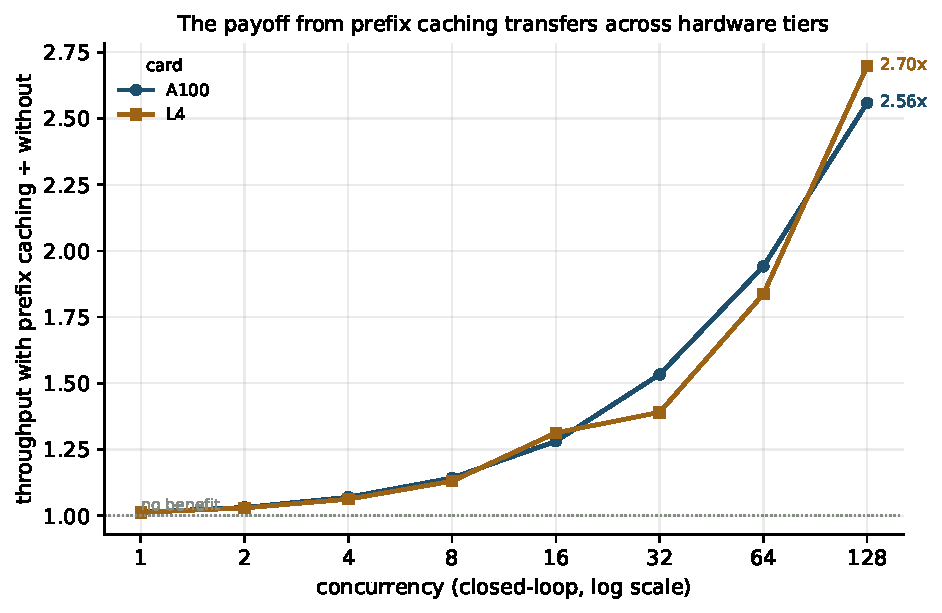
\includegraphics[width=0.72\textwidth]{figs/fig2_payoff.pdf}
\caption{Throughput with prefix caching divided by throughput without, per card.
The two curves nearly coincide across a 4.35--5.26\x{} hardware gap.}
\label{fig:payoff}
\end{figure}

\paragraph{Viability does not transfer at all.} Under the SLO fixed before
measurement, the L4 serves \textbf{zero} compliant requests at every concurrency
level under both configurations (Table~\ref{tab:slo}). Its TPOT $p50$ is
56.56\,ms at concurrency 1 --- past the 50\,ms limit before any load arrives.
Caching improves it substantially at high load, 86.51\,ms against 204.57\,ms at
concurrency 128, but never brings it under the threshold. On the A100 the same
setting is worth 2.95\x{} in goodput at concurrency 128 (16.30 $\rightarrow$
48.11), because it holds TPOT at 19.88\,ms where the uncached configuration
reaches 49.08\,ms and begins to fail. The same knob therefore plays a different
\emph{kind} of role on each card: a throughput optimisation on one, and on the
other a halving of per-token latency that still leaves the card unusable.

\begin{table}[htbp]
\centering\small
\caption{TPOT $p50$ (ms) and goodput (req/s) under the SLO of
\S\ref{sec:setup}. Both L4 columns are zero at every level.}
\label{tab:slo}
\begin{tabular}{@{}rrrrrcrrrr@{}}
\toprule
& \multicolumn{4}{c}{TPOT $p50$ (ms)} & & \multicolumn{4}{c}{Goodput (req/s)}\\
\cmidrule(lr){2-5}\cmidrule(lr){7-10}
Conc. & A100 off & A100 on & L4 off & L4 on & & A100 off & A100 on & L4 off & L4 on\\
\midrule
1   & 12.07 & 12.06 & 56.56  & 56.61 & & 0.64  & 0.64  & \textbf{0.00} & \textbf{0.00}\\
2   & 12.10 & 11.97 & 58.13  & 57.68 & & 1.25  & 1.29  & \textbf{0.00} & \textbf{0.00}\\
4   & 12.03 & 11.95 & 58.03  & 58.10 & & 2.41  & 2.58  & \textbf{0.00} & \textbf{0.00}\\
8   & 12.63 & 12.12 & 60.88  & 58.92 & & 4.43  & 5.07  & \textbf{0.00} & \textbf{0.00}\\
16  & 14.09 & 12.42 & 67.71  & 60.37 & & 7.67  & 9.82  & \textbf{0.00} & \textbf{0.00}\\
32  & 18.84 & 13.43 & 87.06  & 65.04 & & 11.80 & 18.20 & \textbf{0.00} & \textbf{0.00}\\
64  & 27.36 & 15.18 & 125.30 & 74.37 & & 15.91 & 32.02 & \textbf{0.00} & \textbf{0.00}\\
128 & 49.08 & 19.88 & 204.57 & 86.51 & & 16.30 & 48.11 & \textbf{0.00} & \textbf{0.00}\\
\bottomrule
\end{tabular}
\end{table}

\begin{figure}[htbp]\centering
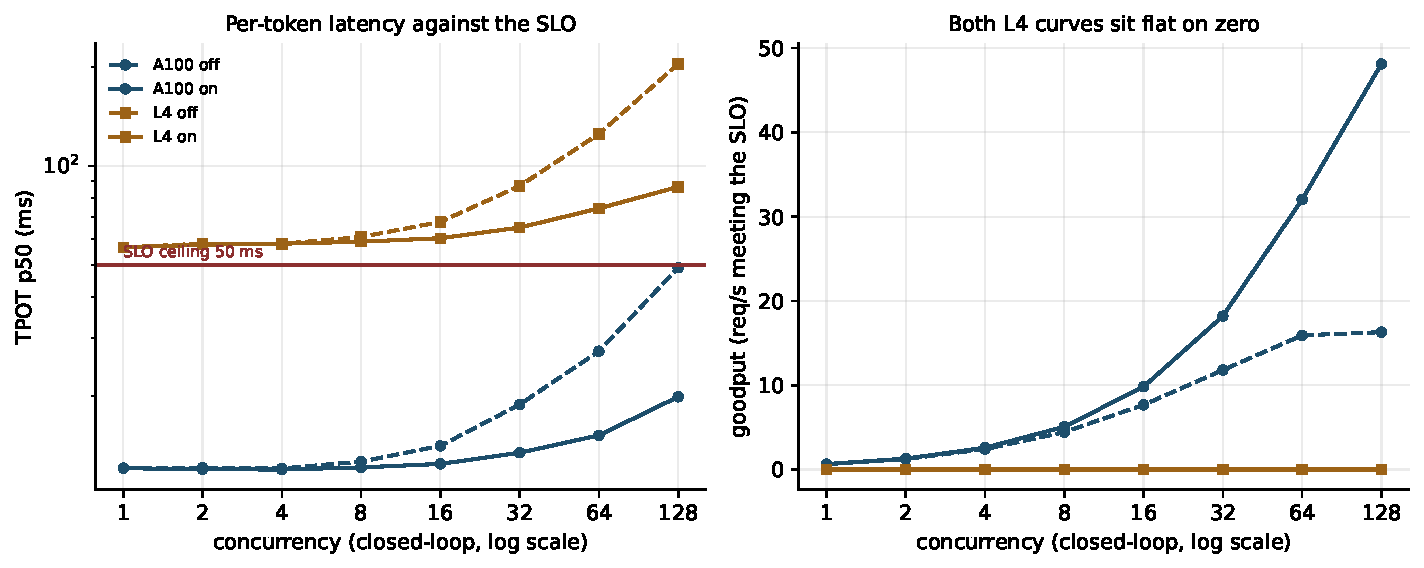
\includegraphics[width=\textwidth]{figs/fig3_slo.pdf}
\caption{Left: per-token latency against the SLO ceiling. Right: goodput. Both
L4 curves sit flat on zero at every concurrency level.}
\label{fig:slo}
\end{figure}

\paragraph{The cost comparison does not survive its own sensitivity check.}
\label{sec:cost}
At GCP list on-demand prices of \$3.67/hr for the A100 40\,GB and \$0.70/hr for
the L4, the L4 delivers 6--20\% more tokens per dollar at every concurrency
level. That ordering is not robust. The break-even A100 price --- the rate at
which the two cards tie, holding the L4 at \$0.70/hr --- is \$3.21--\$3.47/hr
with caching off and \$3.05--\$3.68/hr with it on, so the assumed \$3.67 sits
barely above the range. A $\pm10\%$ swing in the unfavourable direction reverses
the ordering (worst-case minimum ratio 0.87\x{} and 0.82\x{}); even $\pm5\%$
reverses it at some levels. Figure~\ref{fig:cost} therefore plots the break-even
against the assumed price, so a reader can substitute their own contract rate
rather than inherit mine. The defensible statement is that the cost comparison
is too close to call without contract prices.

\begin{figure}[htbp]\centering
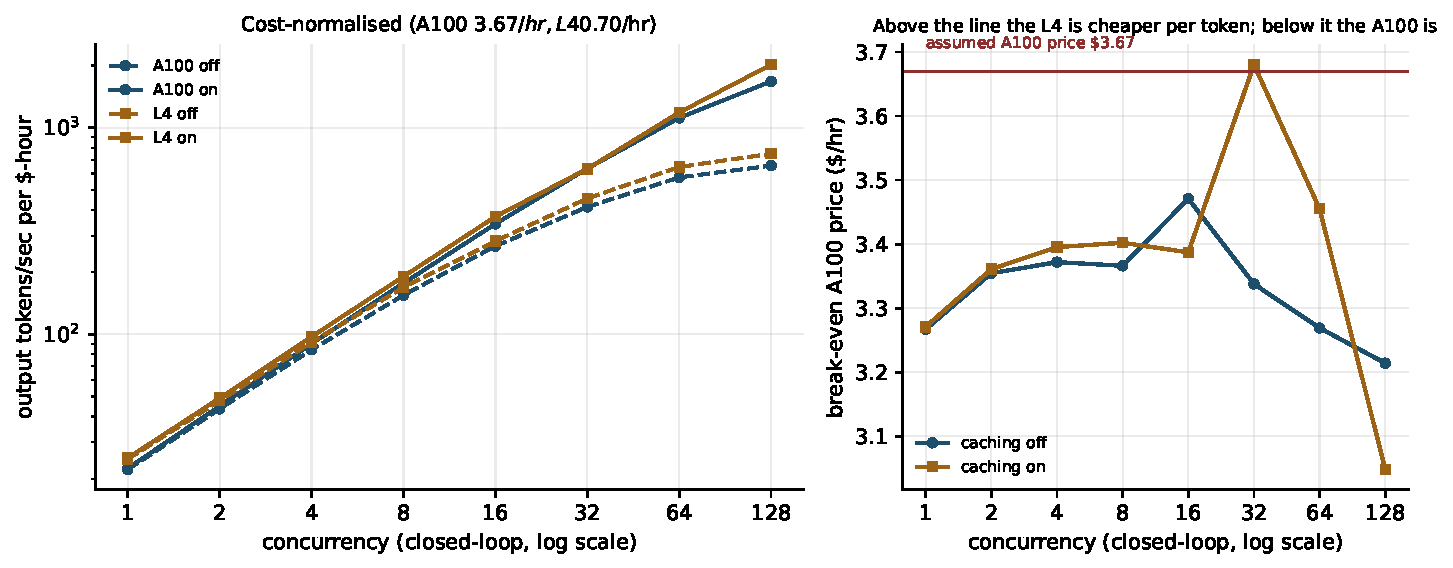
\includegraphics[width=\textwidth]{figs/fig4_cost.pdf}
\caption{Left: cost-normalised throughput. Right: the break-even A100 price at
each concurrency level, against the assumed price.}
\label{fig:cost}
\end{figure}

% ====================================================================
\section{Threats to validity}
\label{sec:threats}
% ====================================================================

\paragraph{Prices are secondary-sourced, and the cost claim rests on them.} The
\$3.67 and \$0.70 figures come from third-party summaries of GCP list pricing,
not from Google's own page, which lists the A100 40\,GB only as part of
\hs{a2-highgpu} machine types rather than as a standalone GPU line item. This is
why \S\ref{sec:cost} reports a break-even range and a sensitivity sweep instead
of a single ratio: the conclusion that follows from these prices is that no
conclusion follows without better ones.

\paragraph{The caching-on curves are a ceiling, not a workload.} Eight prompts
reused hundreds of times per window produce a 96.9\% prefix-cache hit rate,
which is an upper bound on realistic reuse. A production workload with diverse
prompts would sit somewhere between the two curves. The transfer result is
therefore a statement about how the \emph{ceiling} behaves on two cards, not
about a typical deployment.

\paragraph{The L4 verdict is a statement about one SLO.} TTFT $<$ 1000\,ms and
TPOT $<$ 50\,ms were fixed before measurement, but relaxing the latency budget
changes the picture materially.

\begin{table}[htbp]
\centering\small
\caption{Median-request compliance across TPOT budgets. Computed from stored
$p50$ latencies, so this reports whether the \emph{median} request complies
rather than true goodput at each threshold; per-request latencies are not
retained, which is a limitation of the harness rather than of the analysis.}
\begin{tabular}{@{}lllll@{}}
\toprule
TPOT budget & A100 off & A100 on & L4 off & L4 on\\
\midrule
50\,ms  & all levels & all levels & never & never\\
75\,ms  & all & all & never & up to 64\\
100\,ms & all & all & up to 8 & all levels\\
\bottomrule
\end{tabular}
\end{table}

At a 100\,ms budget the L4 becomes viable at every concurrency --- \textbf{but
only with caching on}; without it the L4 fails above concurrency 8. That is a
stronger form of the result: at some latency budgets the configuration is not an
optimisation on the weaker card but a precondition for using it at all.

\paragraph{One curve's configuration is not confirmed by the server's own log.}
The A100 caching-off run's server log was not retained, so
\hs{enable\_prefix\_caching=False} for that curve rests on the launcher's
default at that git SHA rather than on vLLM's own startup banner, which is
available for the other three. The behavioural evidence is strong --- that curve
differs from the caching-on curve by 2.56\x{} at concurrency 128 --- but it is
inference. This matters because a closely related failure did occur during the
L4 pass: a server launched onto an occupied port died with \hs{EADDRINUSE} while
the health check was answered by the \emph{previous} server, producing a
valid-looking file that was a duplicate of the run it was meant to be compared
against. It was caught only because the on/off ratio came out at exactly
1.00\x{} at all eight levels --- too clean to be physical. The launcher now
refuses to start on an occupied port and fails if the launched process exits,
but the A100 curve predates that guard.

\paragraph{Single provider, shared hardware.} All runs are on Colab Pro, where
hardware is shared and the exact host configuration is not under the user's
control. Absolute throughput figures should be read as indicative. The ratios,
which are the contribution, are internally consistent because both members of
each ratio were measured in the same session on the same allocation.

\paragraph{Two vLLM defaults were not swept.} Chunked prefill and asynchronous
scheduling were left on. Both affect the shape of a concurrency curve, and both
are constant across all four curves so neither can explain any reported
difference --- but the absolute numbers describe vLLM at its defaults rather
than a tuned server.

\paragraph{One model, one size, one sequence-length pair.} 512 input and 128
output tokens set the prefill-to-decode balance, and a different pair would move
the numbers. Not swept; stated as a scope limit rather than defended.

\paragraph{Repeat counts differ across cards} --- 3 on the A100, 2 on the L4 ---
a budget decision taken after observing spread of at most 1.66\%. Narrower than
it should be, and the reason is compute cost rather than principle.

\paragraph{Missing instrumentation.} KV-cache utilisation, peak VRAM, GPU
utilisation and framework version are \hs{null} in every record. KV-cache
utilisation is precisely the diagnostic that would have surfaced the prompt-reuse
problem of \S\ref{sec:setup} automatically, instead of requiring the server's
stdout to be read by hand.

% ====================================================================
\section{Conclusion}
% ====================================================================

\textbf{Tested.} One vLLM serving pipeline, one configuration knob, eight
concurrency levels, two GPU tiers, identical model weights, prompt set, sequence
lengths and code. 80 records, all successful, run-to-run spread at most 1.66\%.

\textbf{Found.} The benefit of prefix caching transfers almost exactly across
the hardware gap --- 1.01\x{} at concurrency 1 rising to 2.56\x{} on the A100
and 2.70\x{} on the L4, tracking each other at every level in between. The
hypothesis, which named a ranking change that would move with the card, does
not survive: caching leads everywhere on both cards, so there is no change point
to move. Against the SLO, however, the A100 complies at every concurrency and
the L4 at none.

\textbf{Consequence.} The relative recommendation transfers; the absolute
viability does not. That separates two questions usually asked together.
\emph{How should I configure the server?} can be answered on whatever card is
available, and the answer will carry. \emph{Can this card serve my workload?}
cannot be answered anywhere but on the card itself, and no amount of
configuration work substitutes for asking it --- on the L4 measured here, the
best available setting more than halves per-token latency and still leaves every
request outside the SLO.

The cost comparison, which was intended to be the headline, is the weakest claim
here: at list prices the cheaper card leads on tokens per dollar by 6--20\%, but
the break-even is close enough that a $\pm10\%$ price movement reverses it. It
is reported with its break-even rather than as a ratio, and the honest reading
is that the question needs contract prices to answer.

% ====================================================================
\appendix

\section{Setup detail}
\label{app:setup}
% ====================================================================

\paragraph{Harness validation.} A load generator unable to sustain 128
concurrent streams would produce a flat curve indistinguishable from server
saturation, so the full sweep was first run against a mock server returning a
canned token stream on a fixed sleep, whose ceiling is known by construction.
Measured throughput tracked linearly with concurrency across the entire
$1\rightarrow128$ range --- ratio to linear between 0.93 and 1.06, with no
downward trend at the top of the axis --- and client CPU never exceeded 51\%
mean. Under real load it peaked at 22.8\%, sampled into every record. The
harness is therefore ruled out as an explanation for the shape of any curve
reported in \S\ref{sec:results}.

\paragraph{Reproduction.}
\begin{lstlisting}
python scripts/serve_vllm.py --card A100-SXM4-40GB --precision fp16
#   add --prefix-caching for the ON curve
python scripts/sweep.py --base-url http://localhost:8000 \
    --framework vllm --card A100-SXM4-40GB --precision fp16 \
    --window-s 60 --repeats 3 --warmup-requests 32 \
    --out results/<name>.jsonl
python scripts/analysis.py --emit markdown
python scripts/plot_results.py
\end{lstlisting}

\paragraph{Numbers are generated, not transcribed.} Every figure in
\S\ref{sec:results} is printed by \hs{scripts/analysis.py} from the record
files. An earlier draft contained three quantities stated more confidently than
the data supported --- a run-to-run spread quoted for one curve and applied to
all four, a throughput ratio quoted as a single value when it varied across
operating points, and a ``triples'' that was 2.95\x. None changed a conclusion,
but all three were prose drifting from the data it described. Generating the
tables from the records removes that failure mode mechanically rather than
relying on care.

\paragraph{Provenance and controls.} Every record carries GPU, driver, CUDA
version, torch version, git SHA, model revision and prompt-set hash. Before
computing anything, the analysis asserts that model, revision, prompt hash,
maximum model length, input and output token counts, sampling mode and precision
are identical across all 80 records, and refuses to run otherwise. The four
curves carry \emph{different} git SHAs (\hs{16f2987}, \hs{fcd053b},
\hs{562a207}, \hs{e3dea24}) because code changed between sessions; the diffs
were checked, and only documentation, result files and the two server-launch
scripts changed. \hs{client.py}, \hs{sweep.py} and \hs{record.py} --- the entire
measurement path --- were untouched across all four.

\paragraph{Installation.} vLLM's PyPI wheel ships CUDA 13 binaries while the
runtime's torch was a CUDA 12.8 build, so \hs{import vllm} failed with
\hs{ImportError: libcudart.so.13}. The library was present on disk
(\hs{nvidia-cuda-runtime 13.3.29}) but its directory was not registered with the
dynamic loader; registering it with \hs{ldconfig} fixed the import without
reinstalling anything. Framework installation being coupled to a CUDA version
the user does not control is a real constraint on rented infrastructure, and one
absent from published framework comparisons.

% ====================================================================
\section{The framework comparison that was abandoned}
\label{app:abandoned}
% ====================================================================

This experiment was first designed as a \emph{framework} comparison: vLLM
against TensorRT-LLM~\citep{tensorrtllm} across the same two cards and the same
concurrency axis. A time limit was set on the attempt before it began --- if
neither card had a serving engine within four days, the framework axis would be
dropped and the configuration axis measured instead --- and a 30-minute
installation spike was run first, so the answer would be cheap whichever way it
went.

TensorRT-LLM 1.2.1 installed successfully in 266 seconds, downgrading torch to
2.9.1 in the process, and then:

\begin{lstlisting}
File "tensorrt_llm/_utils.py", line 47, in <module>
    from tensorrt_llm.bindings import DataType, GptJsonConfig, LayerType
ImportError: libcublasLt.so.13: cannot open shared object file:
             No such file or directory
\end{lstlisting}

Three remedies were attempted and all failed: registering every NVIDIA library
directory with \hs{ldconfig} (the library is genuinely absent, not misplaced);
\hs{pip install nvidia-cublas-cu13} from PyPI, which reports
\hs{Failed building wheel} because the entry has no binary; and the same from
NVIDIA's own index, with identical failure. No engine was built on either card,
so \textbf{no build-time data exists and none is claimed}.

Two things here are results rather than mishaps. First, \textbf{both frameworks
shipped CUDA 13 binaries onto a CUDA 12.8 host and both failed at the dynamic
loader} --- but vLLM's missing dependency was present and merely unregistered,
recoverable in one line, while TensorRT-LLM's was absent with no installable
source. Same failure mode, opposite outcomes. Second, \textbf{TensorRT-LLM 1.2.1
pins torch 2.9.1 while vLLM 0.26.0 requires torch 2.11.0}, so the two cannot
share an environment: running both means two installations, two CUDA stacks and
two instances of this class of problem. That is an operational cost of framework
choice, and framework comparisons do not report it.

The question asked in this report is unaffected by the substitution, because it
was never \emph{which framework wins}; it is whether the answer depends on the
hardware, and a configuration axis tests that as directly.

% ====================================================================
\bibliographystyle{plainnat}
\bibliography{refs}

\end{document}
